\begin{figure}
    \centering
    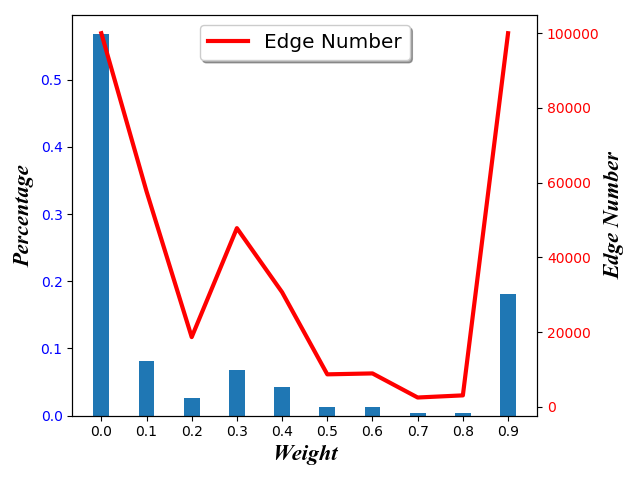
\includegraphics[width=0.48\textwidth]{figs/usenix/rq1weight.png}
    \caption{Distribution of edge weight and the number of edges}
    \label{fig:edgeWeight}
\end{figure}

\subsubsection{RQ1: Graph Reduction Based on Edge Weights or Clustering}
\label{subsubsec:rq1}

With the computed weights for each edge, a straightforward approach to reveal attack sequences is to show only the edges with high weights.
This RQ aims to investigate the feasibility of such approach and the results will motivate the design of \tool.

\myparatight{Statistics of Causality Analysis}
\cref{tab:stasticalSummary} shows the detailed statistics of applying \tool on all the $10$ attack cases. 
As we can see, the average number of nodes and number of edges in the dependency graph are $44,929.8$ and $1,379,446.8$.
After the edge merge in Phase II, the number of edges is still very high ($706,799.6$ on average), while the number of critical edges are only $8.1$ on average, which is consistent with the previous studies~\cite{mcitracking,ma2016protracer,backtracking,backtracking2}.
Thus, it is non-trivial to reveal these edges from the massive non-critical edges by using only weights.

\myparatight{Edge Weight Distribution}
\cref{fig:edgeWeight} shows the edge weight distribution and the corresponding number of edges. Intuitively, the higher-weight edges are more important then the lower-weight edges. Thus, to find critical edges of attack, security analysts will investigate these edges starting from higher weighted edges. But we can see that the average number of high-weighted edges (\ie weights $>0.9$) is as high as $100,000$,
and finding critical edges in such a large dependency graph is still a daunting task for security analysts.

\myparatight{Clustering Results of Edges}
Another approach to reduce the dependency graph is to assign different labels (\ie critical and non-critical) to edges and then only keep edges with the critical label. 
To do so, we applied the Multi-KMeans++ clustering algorithm~\cite{Arthur:2007:KAC:1283383.1283494} to cluster the edges with the computed weights, and the results is shown in \cref{fig:onlyCluster}.
We can clearly see that the smaller cluster consisting of about 6.3\% of total edges. 
If we only keeps the edges belongs to the smaller cluster, the reduced dependency graph will still have more than $40000$ edges, which suffers from the similar problem as using edge weights to hide non-critical edges directly.

Based on our results, we can conclude that the weight-based or cluster-based approach is not sufficient in achieving graph reduction and revealing attack sequences, which provide the motivation for \tool to rank the entry nodes and leverage the forward causality analysis from the top ranked entry nodes for further graph reduction.


\begin{figure}
    \centering
    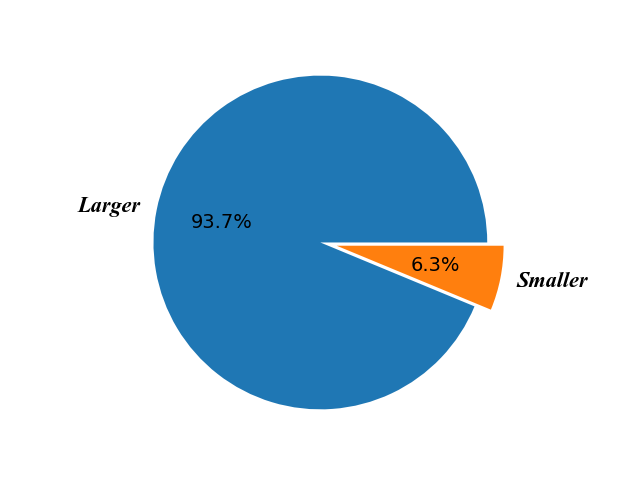
\includegraphics[width=0.48\textwidth]{figs/usenix/cluster.png}
    \caption{Percentage of edges belonging to two clusters}
    \label{fig:onlyCluster}
\end{figure}


  